\section{分支定界闭环检测的原理和实现}


\begin{comment}
1.$\epsilon = [\epsilon_x, \epsilon_y, \epsilon_\theta]^T$表示机器人在地图坐标系下的位姿.
$T_\epsilon$表示位姿估计的坐标变换.


\end{comment}
\begin{frame}
\frametitle{算法原理 \hfill 
\includegraphics[height=0.5cm]{logo.png}}

在Local SLAM中,通过Submap中的Scan-to-Map匹配得到了一个比较理想的机器人位姿估计.
但是由于Local SLAM只使用了一段时间内的局部信息,所以定位误差会随时间积累.
为了能够进一步降低局部累积误差的影响,Cartographer通过Pixel-accurate扫描匹配来进行回环检测,进一步优化机器人的位姿估计.

~\\

%\hspace*{\fill}

计$H=\{h_1, ..., h_k, ..., h_K\}$为传感器扫描到K个hit点集合,$h_k$是第k个hit点在机器人坐标系下的位置坐标.那么$h_k$在地图坐标系下的坐标可以表示为:

\begin{equation}
	T_\epsilon h_k = 
	\begin{bmatrix}
	\cos{\epsilon_\theta } & -\sin\epsilon_\theta \\
	\sin\epsilon_\theta & \cos\epsilon_\theta 
	\end{bmatrix}
	h_k +
	\begin{bmatrix}
	\epsilon_x \\ \epsilon_y
	\end{bmatrix}
\end{equation}

Pixel-accurate扫描匹配问题可以用下式描述:

\begin{equation}
	\epsilon ^* = \mathop{argmax}\limits_{\epsilon \in W} \sum_{k=1}^K M_{nearest}(T_\epsilon h_k)
\end{equation}

式中,$W$是一个搜索窗口,$M_{nearest}(T_\epsilon h_k)$是离$T_\epsilon h_k$最近的栅格单元的占用概率.
可以解释为,在搜索窗口$W$中找到一个最优的位姿,使得hit点集合出现的概率最大化.

%~\\



\end{frame}


\begin{frame}[fragile]
\frametitle{暴力搜索方法}

\begin{columns}
	\column{0.4\textwidth}	
		有一种暴力搜索的方法,如右图所示,这是一种枚举的方法.
		给定搜索步长$r$和$\delta_\theta$,搜索过程以$\epsilon_0$为中心,通过三层循环遍历所有的Pixel并选出得分最高的位姿作为输出$\epsilon^*$
	\column{0.5\textwidth}
暴力匹配的algorithm如下:
\begin{algorithmic}[1]
\State \textbf{Algorithm 1} Naive algorithm for (BBS)
\State $best\_score \leftarrow - \infty$
\State $\text{for } j_x = -w_x \text{ to } w_x \text{ do}$
\State \quad $\text{for } j_y = -w_y \text{ to } w_y \text{ do}$
\State \qquad $\text{for } j_\theta = -w_\theta \text{ to } w_\theta \text{ do}$
\State \qquad \quad $score \leftarrow \sum_{k=1}^K M_{nearset} (T_{\xi 0}+(rj_x,rj_y,\delta_\theta rj_\theta)h_k)$
\State \qquad \quad $\text{if } score > best\_score \text{ then}$
\State \qquad \qquad $match \leftarrow \xi 0 + (rj_x,rj_y,\delta_\theta rj_\theta)$
\State \qquad \qquad $best\_score \leftarrow score$
\State \qquad \quad end if
\State \qquad end for
\State \quad end for
\State end for
\State return $best\_score \text{ and } match \text{ when set.}$
\end{algorithmic}
\end{columns}

\end{frame}

\begin{comment}

\end{comment}
\begin{frame}
\frametitle{分支定界方法 \hfill 
\includegraphics[height=0.45cm]{logo.png}}
\begin{columns}
	\column{0.4\textwidth}
		
	\begin{itemize}
		\item 暴力搜索方法中如果搜索窗口过大或者搜索步长太小,都将导致整个搜索过程耗时过长.
		\item Cartographer使用分支定界方法搜索,该算法的基本思想是:
		\begin{itemize}
			\item 用一颗树表示整个解空间.%,其根节点代表整个搜索窗口$W$.
			\item 每一个节点的孩子都是对该节点所代表的搜索空间的一个划分.
			\item 每个叶节点都对应着一个解.
		\end{itemize}
	\end{itemize}
	
	\column{0.4\textwidth}
	整个搜索过程的基本思想:
	\begin{itemize}
		\item 不断地分割搜索空间,这个过程称为{\color{red}分支}.
		\item 为每次分支之后的孩子节点确定一个上界,这个过程称为{\color{red}定界}.
		\item 如果一个节点的定界超出了已知最优解的值,这意味着该节点下的所有解都不可能比已知解更优,将不在分支该节点.
		%缩小搜索范围,提高算法效率
	\end{itemize}
\end{columns}

\end{frame}

\begin{frame}[fragile]
\frametitle{branch and bound}
分支定界algorithm如下:
\begin{columns}
	\column{0.5\textwidth}
	\begin{algorithmic}[1]
		\State \textbf{Algorithm 2} DFS branch and bound scan matcher for (BBS)
		\State $best\_score \leftarrow score\_threshold$
		\State Compute and memorize a score for each element in $\mathcal{C}_0$.
			   Initialize a stack $\mathcal{C}$ with $\mathcal{C}_0$ sorted by score,
			   the maximum score at the top.
		\State $\textbf{while } \mathcal{C } \text{ is not empty} \textbf{ do}$
		\State \quad $\text{Pop } c \text{ from the stack } \mathcal{C}.$
		\State \quad $\textbf{if } score(c) > best\_score \textbf{ then}$
		\State \qquad $\textbf{if } c \text{ is a left node } \textbf{then}$
		\State \qquad \quad $match \leftarrow \xi_c$
		\State \qquad \quad $best\_score \leftarrow score(c)$

		
	\end{algorithmic}
	
	\column{0.5\textwidth}
	\begin{algorithmic}[1]
		\State \qquad \textbf{else}
		\State \qquad \quad Branch: Split $c$ int nodes $\mathcal{C}_c$.
		\State \qquad \quad Compute and memorize a score for each element in $\mathcal{C}_c$.
		\State \qquad \quad Push $\mathcal{C}_c$ onto the stack $\mathcal{C}$, 
							sorted by score, the 
							\Statex \qquad \quad maximum score last.
		\State \qquad \textbf{end if}
		\State \quad \textbf{end if}
		\State \textbf{end while}
		\State return $best\_score $ and $match$ when set.
		
	\end{algorithmic}
\end{columns}
\end{frame}


\begin{frame}[fragile]
\frametitle{branch and bound}
分支定界algorithm如下:
\begin{columns}
\column{0.5\textwidth}
\begin{algorithmic}[1]
\State \textbf{Algorithm 2} Generic branch and bound
\State $best\_score \leftarrow - \infty$
\State $\mathcal{C} \leftarrow \mathcal{C}_0$
\State $\textbf{while } \mathcal{C} \neq \emptyset \textbf{ do}$
\State \quad $\text{Select a node } c \in \mathcal{C} \text{ and remove it from the set.}$
\State \quad $\textbf{if } c \text{ is a left node } \textbf{then}$
\State \qquad $\textbf{if } score(c) > best\_score \textbf{ then} $
\State \qquad \quad $solution \leftarrow n$
\State \qquad \quad $best\_score \leftarrow score(c)$
\State \qquad \textbf{end if}
\State \quad \textbf{else}
\State \qquad $\textbf{if } score(c) > best\_score \textbf{ then}$
\State \qquad \quad Branch: Split $c$ into nodes $\mathcal{C}_c$.
\State \qquad \quad $\mathcal{C} \leftarrow \mathcal{C} \cup \mathcal{C}_c$

\end{algorithmic}

\column{0.5\textwidth}
\begin{algorithmic}[1]

\State \qquad \textbf{else}
\State \qquad \quad Bound.
\State \qquad \textbf{end if}
\State \quad \textbf{end if}
\State \textbf{end while}
\State return $best\_score $ and $solution$ when set.

\end{algorithmic}

\end{columns}
\end{frame}


\begin{comment}

\end{comment}
\begin{frame}
\frametitle{分支定界方法 \hfill 
\includegraphics[height=0.5cm]{logo.png}}

\begin{columns}
	\column{0.5\textwidth}
	
	\begin{itemize}
		\item 搜索窗口的栅格索引集合$\overline{\mathcal{W}}$可以通过笛卡尔积$\{-w_x, ..., w_x \} \times 
		\{-w_y, ..., w_y \} \times \{-w_\theta, ..., w_\theta \}$来枚举.
		其中,$w_x$, $w_y$分别是$x$和$y$方向上最大的索引, $w_\theta$是角度的最大索引.
		
		%\hspace*{\fill}
		
		\vspace{0.3cm} %调节垂直间距,正数表示加大间距,负数表示缩小间距
		%\hspace{-0.15cm}
		
		\item 搜索窗口$\mathcal{W}$可以用集合$\{\epsilon_0 + (rj_x, rj_y, \delta_\theta j_\theta) \in \overline{\mathcal{W}} \}$来表示.
		其中,$\epsilon_0$是搜索的中心,也是机器人位姿的初始估计. $r$ 和$\delta_\theta$分别是位移和角度的搜索步长.
	\end{itemize}
	
	\column{0.5\textwidth}
	\begin{itemize}
		\item 搜索树中每个节点都可以用是个整数$c=(c_x, c_y, c_\theta, c_h) \in \mathbb{Z}^4$来表示. 其中,$c_x$, $c_y$分别是搜索空间$x, y$轴的起始索引, $c_{\theta}$是搜索角度, $c_h$代表该搜索空间有$2^{c_h} \times 2^{c_h}$个可能的解.它们具有相同的角速度,但位置坐标不同.这些解的组合可以用如下的笛卡尔积来表示:
		\vspace{0.2cm}
		\begin{equation}
			\overline{\mathcal{V}_c} = \{(j_x, j_y) \in \mathbb{Z}^2 | 
			\begin{matrix}
			c_x \leq j_x < c_x + 2^{c_h} \\
			c_y \leq j_y < c_y + 2^{c_h}
			\end{matrix}
			\}
		\end{equation}
	\end{itemize}
\end{columns}

\end{frame}

\begin{comment}
\end{comment}
\begin{frame}
\frametitle{分支定界方法 \hfill 
\includegraphics[height=0.5cm]{logo.png}}

\begin{columns}
	\column{0.7\textwidth}
	
	\begin{itemize}
		\item 该节点对应搜索空间的栅格索引集合为$\overline{W_c} = \overline{\mathcal{V}_c} \cap \overline{\mathcal{W}}$.
		%\vspace{0.2cm}
		\item 每当对节点进行分支,就相当于在空间坐标上将搜索空间划分为四个区域,如右图所示.
		\item 对于叶子节点而言,$c_h = 0$,其搜索空间中只有一个索引对应着解$\epsilon_c = \epsilon_0+(rc_x, rc_y, \delta_\theta c_\theta)$.
		\item 如果指定搜索树的高度$h_0$,那么初始子空间节点集合中的节点$c \in \{C_0\}$的四个整数可以表示为:
		\vspace{0.2cm}
		\begin{equation}
			c = 
			\begin{cases}
			c_x = -w_x + 2^{h_0}j_x \qquad : j_x \in \mathbb{Z}, 0 \leq 2^{h_0}j_x \leq 2w_x \\
			c_y = -w_y + 2^{h_0}j_y \qquad : j_y \in \mathbb{Z}, 0 \leq 2^{h_0}j_y \leq 2w_y \\
			c_\theta = j_\theta \qquad\qquad\qquad\ : j_\theta \in \mathbb{Z}, -w_\theta \leq j_\theta \leq w_\theta \\
			c_h = h_0 \
			\end{cases}
		\end{equation}
	\end{itemize}
	
	\column{0.3\textwidth}
	\begin{figure}[h]
		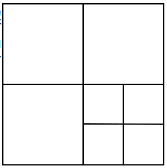
\includegraphics[trim=1.5 0 0 0, height=3.5cm,clip]{carto/4dtree.png}
		\caption{四个区域搜索空间}
	\end{figure}
\end{columns}

\end{frame}

\begin{comment}
\end{comment}
\begin{frame}
\frametitle{分支定界方法 \hfill 
\includegraphics[height=0.5cm]{logo.png}}
\begin{columns}
	\column{0.5\textwidth}
	\begin{itemize}
		\item 搜索树上的每个节点的上界可以通过下式计算得到:
		\vspace{0.2cm}
		\begin{equation}
			\begin{array}{lcr}
			 score(c)  & = &  \sum_{k=1}^K \mathop{max}\limits_{j \in \overline{\mathcal{V}_c}} M_{nearest(T_{\epsilon_j}, h_k)} \\
			 & \geq &\sum_{k=1}^K \mathop{max}\limits_{j \in \overline{\mathcal{W}_c}} M_{nearest(T_{\epsilon_j}, h_k)} \\
			 &\geq& \mathop{max}\limits_{j \in \overline{\mathcal{W}_c}} \sum_{k=1}^K M_{nearest(T_{\epsilon_j}, h_k)} 
			 \end{array}
		\end{equation}
		\item 如果对每一个节点都直接计算上界的话,将是一个很大的计算量.
		Cartographer采用一种类似图像金字塔的方法,{\color{red}预先计算出占用栅格地图在不同分支尺寸下的上界},
		在实际计算上界时只需要根据$c_h$查询对应尺度下的占用栅格即可获得节点的上界.右图是分支尺寸分别为1,4,16,64时的占用概率上界.
	\end{itemize}
	\column{0.4\textwidth}
	\begin{figure}[h]
		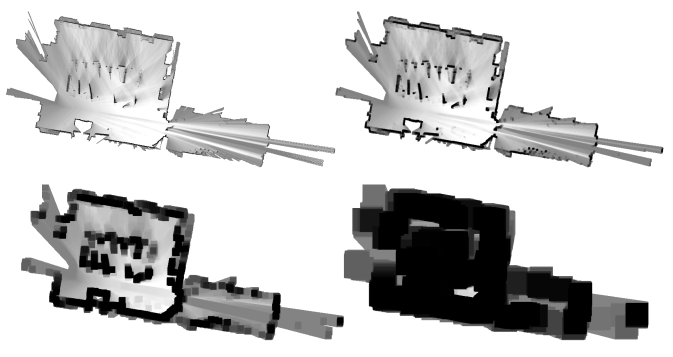
\includegraphics[trim=0 0 0 0, height=3.5cm,clip]{carto/precomputed_grid.png}
		\caption{分支尺寸分别为1/4/16/64时的占用概率上界}
	\end{figure}
\end{columns}
\end{frame}

\begin{comment}
\end{comment}
\begin{frame}
\frametitle{分支定界方法 \hfill 
\includegraphics[height=0.5cm]{logo.png}}
\begin{columns}
	%\column{0.1\textwidth}
	\column{0.7\textwidth}
	\begin{itemize}
		\item 我们称这个图为预算图,对于第$h$层的节点,在预算图中$x,y$的占用上界可以表示成下式,即以考察点$x,y$为中心,
		尺寸为$2^h \times 2^h$的窗口内栅格的最高占用概率为上界.
		\begin{equation}
			M_{precomp}^h(x,y) = \mathop{max}\limits_{
			\begin{matrix}
			x^\prime \in [x, x+r(2^h-1)]\\
			y^\prime \in [y, y+r(2^h-1)] 
			\end{matrix}}
			M_{nearest}(x^\prime, y^\prime)
		\end{equation}
		\vspace{0.2cm}
		\item 节点c的上界可以直接查表得到:
		\begin{equation}
			score(c) = \sum_{k=1}^K M_{precomp}^{c_h}(T_\epsilon h_k)
		\end{equation}
		\vspace{0.2cm}
		\item 整个闭环检测的业务逻辑是:根据当前的子图构建一个占用栅格地图,然后为该地图计算预算图,
		接着通过深度优先的分支定界搜索算法估计机器人的位姿,最后建立机器人位姿与子图之间的约束关系.
	\end{itemize}
%	\column{0.1\textwidth}

\end{columns}
\end{frame}


\begin{comment}
\end{comment}
\begin{frame}
\frametitle{分支定界方法 \hfill 
\includegraphics[height=0.5cm]{logo.png}}
\begin{columns}
	\column{0.3\textwidth}
	\begin{itemize}
		\item 把全部可行解空间反复分割为越来越小的子集,称为{\color{red}分支}.
		\item 对每个子集内的解集计算一个目标下界(对于最小值问题),称为{\color{red}定界}.
		\item 在每次分支后,凡是界限超出已知可行解集目标值的那些子集不再进一步分支,这样,许多子集可不予考虑,这称为{\color{red}减枝}.
		\item 分支定界法中,通过分支/定界/剪枝操作,使我们仅在一部分可行解中寻找最优解,而不是全部穷举出来在寻找,求解效率更高.
		%\vspace{0.3cm}
	\end{itemize}
	\column{0.7\textwidth}
	以整数规划为例,首先规定求解的整数规划问题为A,相应的线性规划问题为B(松弛问题).
	\begin{enumerate}
		\item 对问题B进行求解:
		\begin{enumerate}
			\item 若B无可行解,则A也无可行解,停止计算.
			\item 若B有最优解,且符合整数条件,该最优解为A的最优解,停止计算.
			\item 若B有最优解,但不符合整数条件,计它的目标函数值为$z^*$作为最优解的{\color{red}下界}.
		\end{enumerate}
%		\vspace{0.5cm}
		\item 找出问题A的一个可行解,其目标函数值作为最优解的{\color{red}上界}.
		\item 迭代:
		\begin{enumerate}
			\item 分支,在B中的最优解中人选一个不符合整数条件的变量$x_j$,其值为$b_j$,构造两个约束条件,$x_j \leq [b_j], x_j \geq [b_j] + 1$,分别加入到问题B中,形成两个子问题B1和B2.不考虑整数条件求解这两个子问题.
			\item 定界, 对每个后续问题表明其求解结果,与其他问题进行比较,将最优目标函数值最小者(不包括问题B)作为新的下界,
			在已符合整数条件的各分支中,找出目标函数值最小者作为新的上界.
			\item 剪枝,将目标函数不在下界和上界中的分支剪去.
			\item 重复123,直到得到最优解.
		\end{enumerate}
	\end{enumerate}

\end{columns}
\end{frame}

\begin{comment}
\end{comment}
\begin{frame}
\frametitle{分支定界方法 \hfill 
\includegraphics[height=0.5cm]{logo.png}}
\begin{columns}
	\column{0.6\textwidth}
	\begin{itemize}
		\item Cartographer使用类FastCorrelativeScanMatcher2D具体实现了深度优先的分支定界搜索算法,
		该算法能够高效地确定激光点云与子图的匹配度,估计采样点云时机器人相对于子图的位姿.
		为了能够高效的对搜索空间进行分割并计算上界,Cartographer还为每个子图计算了不同尺度下的占用概率,
		以后的搜索过程只需要简单的查表就可以完成.

	\end{itemize}

\end{columns}
\end{frame}

%%%%%%%%%%%%%%%%templete%%%%%%%%%%%%%%%%%%%%%
\begin{comment}
\end{comment}
\begin{frame}
\frametitle{分支定界方法 \hfill 
\includegraphics[height=0.5cm]{logo.png}}
\begin{columns}
	\column{0.5\textwidth}
	\begin{itemize}
		\item 
		\vspace{0.2cm}
		\item 
	\end{itemize}
	\column{0.5\textwidth}
	\begin{itemize}
		\item 
		\vspace{0.5cm}
		\item
	\end{itemize}
\end{columns}
\end{frame}

%%%%%%%%%%%%%%%%templete%%%%%%%%%%%%%%%%%%%%%

\begin{frame}[fragile]
\frametitle{branch and bound}
\end{frame}



\begin{frame}
\frametitle{branch and bound}
回环检测是一种匹配过程,即当获得新的scan时,再其附近一定范围内搜索最优匹配帧,若该最优匹配帧符合要求,则认为是一个回环.该匹配问题可以描述为以下式子.
\begin{equation}
\xi ^* = \mathop{argmax}\limits_{\xi \in W} \sum_{k=1}^K M_{nearest}(T_\xi h_k) \qquad (BBS)
\end{equation}

其中$W$是搜索空间,$M_{nearest}$是该点对应栅格点的$M$值.该式子可以理解为对于scan中的每一个光束映射到该地图中某个submap的某个laser scan上时的置信度和,置信度越高则认为越相似,我们需要在$W$空间中寻找出该置信度和最大的submap.

\end{frame}
